\chapter{Progetto e attività di stage}
\textit{Questa capitolo parla delle attività di stage andando a descrivere il progetto nei suoi stati di avanzamento, le scelte adottate e le motivazioni che mi hanno permesso di scegliere.}

\section{Formazione}
All'inizio dello stage, la prima attività che ho dovuto svolgere è stata quella di studio delle applicazioni adottate dall'azienda e i formalismi, ovvero codici e abbreviazioni adottate per la realizzazione dei campi di database. 
Per la formazione sull'applicazione \inde\, ho seguito sei video-corsi della durata di una o anche due ore l'uno. In aggiunta, per velocizzare l'apprendimento dell'uso dell'applicazione, è stato richiesto che venissero realizzate le applicazioni presenti nei video.
Rispetto a quanto pianificato, l'apprendimento del programma è risultato più rapido della settimana preventivata e quindi, durante la stessa, ho potuto interfacciarmi con i data warehouse e lo studio di alcune stored procedure. 
Verso fine settimana ho iniziato lo studio dei documenti relativi al configuratore catalogo/prodotti.


\section{Progettazione}
Dalla seconda settimana di stage, ho iniziato ad affrontare le dinamiche aziendali concentrandomi nelle attività di progetto che è stata divisa in incontri con il cliente e lavoro presso la sede di Castelfranco.

\subsection{Database}
Affiancato al tutor aziendale, il primo punto affrontato è stato il database. Il cliente ci ha dato carta bianca, ovvero potevamo decidere tra due soluzioni: riutilizzare tabelle presenti nel database oppure crearne di nuove. Questo cliente specifico dispone tra i suoi software di sei applicazioni ideate con InDe e nei mesi di stage hanno iniziato a chiedere nuovi progetti.

La scelta, dopo una attenta discussione con il cliente, è stata quella di creare delle tabelle nuove perché questa nuova componente in futuro vorrebbero integrarla in altre applicazioni oltre che a quella per cui è stata realizzata.\\
Per cercare di mantenere una certa uniformità con il resto del data warehouse, la prima scelta è stata quella di non inserire vincoli di Foreign Key.
Questo vincolo che avrebbe permesso query più rapide è risultato superfluo in seguito alla velocità dei server. Tuttavia, continuo a ritenere molto utile la creazione delle foreign key perché in questo modo se anche le tabelle iniziano ad avere una quantità di record spropositata la velocità resta soddisfacente. Inoltre, il problema dell'eventuale plugin dell'applicazione richiede comunque che si metta mano al codice nell'importazione della componente. 
Quest'ultima scelta ha portato il vantaggio di estendere i progetti in maniera più rapida.
Infine, per concludere il tema vincoli gli unici adottati sono quelli di Primary Key.
\\

La prima tabella da cui partire è quella dedicata agli articoli. Quest'ultima è già presente nel data warehouse e dispone di una vista. Partendo da questi due contenitori, si è realizzata una struttura che permetta prima di realizzare una lista prodotti, poi, se l'articolo esiste, arricchire le sue informazioni.\\

Gli aspetti da tenere in considerazione sono stati:
\begin{itemize}
	\item ogni articolo ha delle immagini, video o dei file di vario genere;
	\item ogni articolo deve poter avere uno o più tag;
	\item ogni articolo deve avere delle informazioni di base e delle informazioni aggiuntive;
	\item ogni informazione aggiuntiva deve poter essere gestita (creata, modificata ed eliminata).
\end{itemize}
Queste informazioni sono state definite durante la prima riunione presso la sede del cliente.\\

\begin{figure}[!h] 
	\centering 
	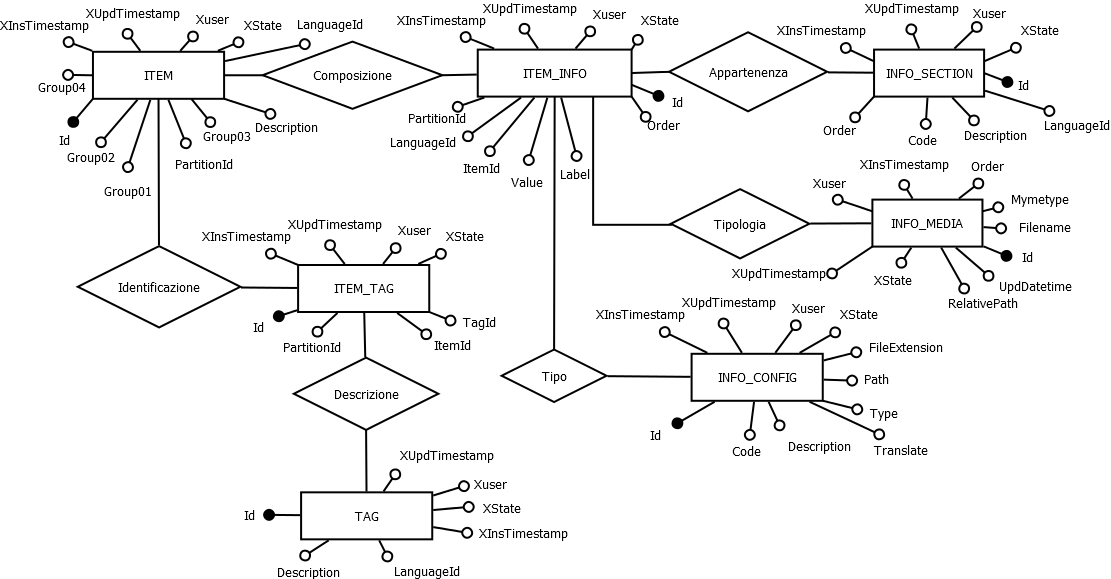
\includegraphics[width=1\columnwidth]{DiagrammaER} 
	\caption{Diagramma Entity Relationship}
	\label{DiagrammaER}
\end{figure}

Il diagramma ER (i vincoli sono fittizi, mostrano i collegamenti nonostante l'assenza di foreign key) è stato pensato in modo tale che ogni articolo dispone di molte informazioni e ciascuna di esse appartiene ad una categoria.

\paragraph{ITEM}
Questo oggetto è una vista con alcune delle informazioni più importanti. Visto che la fase di inserimento prevede unicamente che un'utente possa inserire alcune informazioni. I dati gestiti nella vista sono i gruppi di appartenenza (ad esempio insaccati, surgelati, prodotti da forno) ed una descrizione breve dell'oggetto.
In questo contesto la descrizione appare due volte una negli ITEM ed una nella ITEM\_INFO per il semplice motivo che la tabella esisteva già nel database.

\paragraph{ITEM\_INFO}
Nella seguente tabella vengono raccolte tutte le informazioni e rappresenta il punto di collegamento dell'intero progetto. In esso vengono inserite le etichette e i valori che rappresentano i punti fondamentali di questa tabella. Le etichette (label) sono la descrizione dei valori (value) che permettono ricerche in tabella più rapide (video, titolo, immagine). I valori sono quelli che in base alle altre tabelle saranno stampati a video dall'applicazione web di front-end (\hyperref[frontend]{figura \ref{frontend}}).

\paragraph{INFO\_CONFIG}
La tabella INFO\_CONFIG è stata realizzata al fine di inserire record con specifiche che limitano i tipi di record che possono essere gestiti all'interno di ITEM\_INFO. Inoltre definiscono le caratteristiche su cui sono fondati i record della tabella associata ad esempio è possibile definire le estensioni di file o un parametro che mi hanno chiesto di gestire in un secondo momento, ovvero la lingua; nel diagramma risulta già presente, ma in realtà è stato aggiunto in un secondo momento verso fine progetto circa a metà della penultima settimana.

\paragraph{INFO\_MEDIA}
INFO\_MEDIA è la tabella, come è comprensibile dal nome, che detiene tutte le informazioni relative ai file. In questo caso una prima idea è stata quella di salvare il file nel database con un blob, tuttavia ho pensato che poi nell'interrogazione di una tabella contenente molti media poteva diventare molto pesante considerando la richiesta di gestione dei video. In questa occasione ho pensato fosse più propizio ideare una cartella online dove è installata l'applicazione con un GUID (nome univoco) assegnato al file e nel database disporre unicamente del percorso relativo dell'immagine.

\paragraph{INFO\_SECTION}
Le informazioni relative ad un prodotto devono essere categorizzate. Questa tabella ha la funzione di indicare la categoria di appartenenza così come avviene in diversi siti e-commerce. L'idea è di poter gestire le informazioni presentandole in sezioni dinamiche tante quante si ritengano necessarie. 

\paragraph{TAG}
Tabella che serve ad includere ogni tipo di parole chiavi che permettano di effettuare ricerche per arrivare ad uno specifico prodotto o gruppo di prodotti. Questa tabella non è stata creata perché è adoperata in altri contesti.

\paragraph{ITEM\_TAG}
Quest'ultima tabella ha lo scopo di collegare i tag con lo specifico articolo. Si è di fronte ad una relazione uno a molti che, in fase di ristrutturazione, ha comportato la creazione di una tabella intermedia tra articoli e tag.



\subsection{Design Pattern}
Nella realizzazione dell'applicazione per la maggior parte delle videate un singolo oggetto doveva gestire le sue operazioni nella propria videata. Vi è stato solo un caso particolare che ha richiesto l'uso di un design pattern e che già nella fase di progettazione del database è stato abbozzato: nella gestione di dettaglio del singolo articolo.
Il pattern scelto è il Facade. Tutte le informazioni partono da un articolo (record della tabella ITEM) e da questo vengono generate opportune operazioni.\\

\begin{figure}[!h] 
	\centering 
	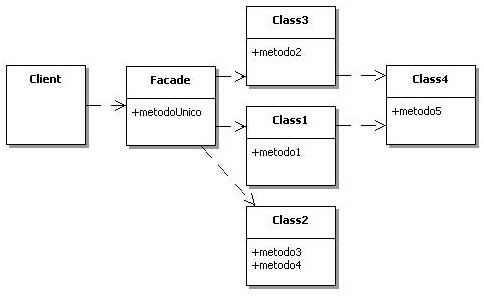
\includegraphics[width=1\columnwidth]{Pattern} 
	\caption{Design pattern strutturale: Facade}
	\label{Pattern}
\end{figure}


Il grafico UML generato una volta definito il design pattern da applicare è risultato essere quello sottostante. Per realizzarlo, ho seguito la logica che doveva avere l'applicazione ed ho provato a segnare le attività di caricamento, creazione, modifica e cancellazione dei record delle diverse tabelle.

\begin{figure}[!h] 
	\centering 
	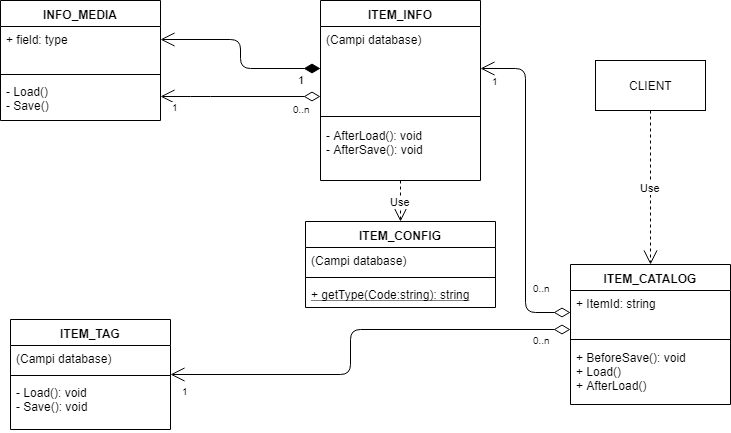
\includegraphics[width=0.7\columnwidth]{UML} 
	\caption{Diagramma UML delle classi}
	\label{UML}
\end{figure}

%\subsubsection{Diagrammi di sequenza}
\paragraph{Caricamento}
Un dettaglio articolo non è altro che un'insieme di informazioni (ITEM\_INFO). Partendo da questo presupposto ho deciso di caricare un array di oggetti (in InDe prende il nome di IDCollection).
Per definire quale articolo caricare indico uso l'id dell'articolo; quindi carico le varie informazioni tramite query. Quando ricevo una informazione verifico immediatamente a quale configurazione (INFO\_CONFIG) appartiene e solo se necessario carico gli ulteriori dati, ovvero i media. Infine, con la classe ITEM\_TAG metto in un array tutti i tag associati all'articolo selezionato.

\paragraph{Creazione}
Questa operazione è molto più semplice e controllata. Prima creo un articolo (ITEM), quindi entro nel dettaglio e creo tanti ITEM\_INFO con o senza il proprio ITEM\_MEDIA. Poi se vengono inseriti creo gli ITEM\_TAG. Tutto questo viene salvato unicamente dall'oggetto ITEM\_CATALOG che fa partire gli eventi di save dei vari oggetti.

\paragraph{Modifica}
In questo caso la modifica è uguale all'inserimento. La differenza è che in inserimento all'inizio devo creare un articolo e poi aprire il suo dettaglio senza caricare informazioni. In questa situazione, l'oggetto deve caricare ogni singola informazione quindi è necessario un controllo sulle query se ritornano o meno informazioni. In seguito, cambiando un dato questo segnala all'oggetto, a volte forzando l'update, che devono essere aggiornati i dati.

\paragraph{Cancellazione}
L'ultima operazione non meno importante è la cancellazione. Questa deve generare la cancellazione di ogni singolo record di uno specifico articolo senza lasciare record "orfani". Per evitare questo fenomeno, quando cancello inizio dai figli fino al raggiungimento del padre ed infine blocco la cancellazione dell'articolo (ITEM), ma cambio lo stato di un campo del record da "I" (Insert) o "M"(Modified) a "D" (Deleted) ed aggiorno XUpdDatetime.

\section{Codifica}
Dopo la fase di progettazione, si è affrontata la codifica. Questa fase è stata differente rispetto a quanto ho sviluppato durante il corso di Programmazione ad oggetti, Programmazione concorrente e distribuita ed Ingegneria del Software. Il motivo della diversità è l'applicazione \inde\.\\
Progettare classi e videate con questo software mi hanno abbastanza cambiato il modo di implementare e testare. Prima di questo cambiamento tendevo a crearmi una scaletta, implementarla e passo per passo effettuare dei test di unità basati su codice scritto (ad esempio Java associato a JUnit).\\
In questo contesto, invece, mi sono ritrovato a saltare i test di unità e passando immediatamente a test di sistema. Di conseguenza creavo classi, metodi ed eventi cercando quanto più possibile di seguire una logica rigorosamente commentata. Mi attendevo molti errori, ma sono rimasto sorpreso. Il numero di errori, per il fatto che il codice generato si basa su template ben controllato e già testato dalla casa produttrice, era molto basso e con il debugger incluso ho potuto risolvere ogni errore commesso in poco tempo per poi passare ad altre funzionalità.

\subsection{Classi base}


\subsection{Facade: ITEM\_CATALOG}

\subsection{Videate}
elenco delle videate normali

\subsubsection{Modali}
metodo seguito come le si sono implementate

\section{Verifica, validazione e collaudo}

\section{Altri interventi}

\section{\inde: creazione di una schermata base}
In questa sezione ho desiderio di analizzare, oltre che alla fase di codifica del progetto, il particolare aiuto derivante da InDe. Illustro come una pagina web viene creata da zero per permettere ai lettori di questo documento di comprendere quanto può essere semplice, con l'aiuto di strumenti RAD come questo, creare applicazioni.

\subsection{Passo 1: Database}
\subsection{Passo 2: Oggetto}
\subsection{Passo 3: Videata}
\subsection{Passo 4: Estensioni}



